% Architecture of Phase 3 (load balancer and three servers). Compile with: pdflatex architecture_phase3.tex
\documentclass[tikz,border=1pt]{standalone}
\usepackage{mathptmx}
\usetikzlibrary{positioning,fit,arrows.meta,shapes.geometric,backgrounds,calc}

\begin{document}
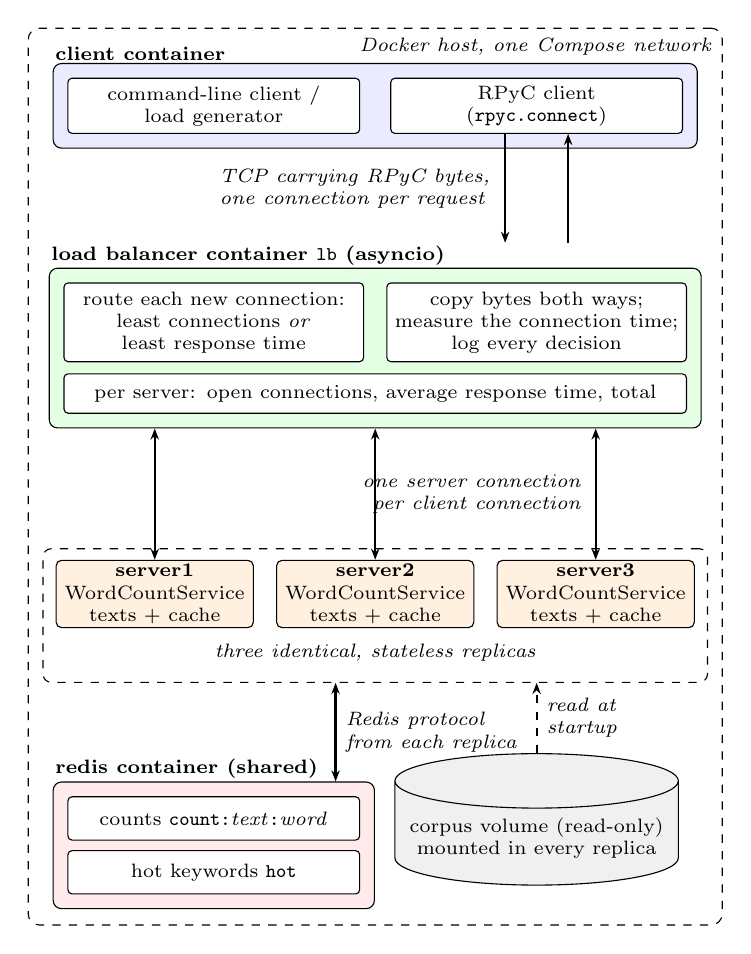
\begin{tikzpicture}[
    >={Stealth[length=4pt,width=3pt]},
    comp/.style={draw, rounded corners=1.5pt, fill=white, align=center, font=\scriptsize,
                 inner sep=1.5pt, minimum height=7mm, text width=#1, minimum width=#1},
    comp/.default=36mm,
    box/.style={draw, rounded corners=3pt, inner sep=1.8mm},
    boxtitle/.style={font=\scriptsize\bfseries, anchor=south west, inner sep=0.8pt},
    note/.style={font=\scriptsize\itshape, align=left, inner sep=1pt},
]
  % ---------------- client tier ----------------
  \node[comp] (cli)  at (2.0, 0) {command-line client /\\load generator};
  \node[comp] (stub) at (6.1, 0) {RPyC client\\(\texttt{rpyc.connect})};
  \begin{scope}[on background layer]
    \node[box, fill=blue!8, fit=(cli)(stub)] (client) {};
  \end{scope}
  \node[boxtitle] (clientT) at (client.north west) {client container};

  % ---------------- load balancer ----------------
  \node[comp=37mm, minimum height=10mm] (route) at (2.0, -2.75)
       {route each new connection:\\least connections \emph{or}\\least response time};
  \node[comp=37mm, minimum height=10mm] (relay) at (6.1, -2.75)
       {copy bytes both ways;\\measure the connection time;\\log every decision};
  \node[comp=78mm, minimum height=5mm, below=1.4mm of $(route.south)!0.5!(relay.south)$] (state)
       {per server: open connections, average response time, total};
  \begin{scope}[on background layer]
    \node[box, fill=green!10, fit=(route)(relay)(state)] (lb) {};
  \end{scope}
  \node[boxtitle] (lbT) at (lb.north west) {load balancer container \texttt{lb} (asyncio)};

  % ---------------- server replicas ----------------
  \foreach \i/\x in {1/1.25, 2/4.05, 3/6.85} {
    \node[draw, rounded corners=2pt, fill=orange!12, align=center, font=\scriptsize,
          text width=24mm, minimum width=24mm, inner sep=1.5pt] (s\i) at (\x, -6.2)
         {\textbf{server\i}\\WordCountService\\texts + cache};
  }
  \node[font=\scriptsize\itshape, below=0.8mm of s2] (groupT) {three identical, stateless replicas};
  \begin{scope}[on background layer]
    \node[draw, dashed, rounded corners=3pt, inner xsep=1.6mm, inner ysep=1.4mm, fit=(s1)(s3)(groupT)] (group) {};
  \end{scope}

  % ---------------- data tier ----------------
  \node[comp, minimum height=5.5mm] (counts) at (2.0, -9.05) {counts \texttt{count:}\textit{text}\texttt{:}\textit{word}};
  \node[comp, minimum height=5.5mm, below=1.2mm of counts] (hot) {hot keywords \texttt{hot}};
  \begin{scope}[on background layer]
    \node[box, fill=red!8, fit=(counts)(hot)] (redis) {};
  \end{scope}
  \node[boxtitle] (redisT) at (redis.north west) {redis container (shared)};
  \node[draw, cylinder, shape border rotate=90, aspect=0.2, fill=gray!12, align=center, font=\scriptsize,
        minimum width=36mm, minimum height=12mm] (corpus) at (6.1, -9.3)
        {corpus volume (read-only)\\mounted in every replica};

  % ---------------- connectors ----------------
  \coordinate (reqTop) at ([xshift=-4mm]stub.south);
  \coordinate (repTop) at ([xshift=4mm]stub.south);
  \draw[->, thick] (reqTop) -- (reqTop |- lbT.north);
  \draw[<-, thick] (repTop) -- (repTop |- lbT.north);
  \node[note, anchor=east] at ($(reqTop)!0.5!(reqTop |- lbT.north) + (-1.5mm, 0)$)
       {TCP carrying RPyC bytes,\\one connection per request};

  \foreach \i in {1, 2, 3} {
    \draw[<->, thick] (lb.south -| s\i.north) -- (s\i.north);
  }
  \node[note, anchor=east, align=right] at ($(lb.south -| s3.north)!0.5!(s3.north) + (-1.5mm, 0)$)
       {one server connection\\per client connection};

  \coordinate (respX) at ([xshift=-5mm]redis.north east);
  \draw[<->, thick] (group.south -| respX) -- node[note, right=0.8mm] {Redis protocol\\from each replica} (respX);
  \draw[->, thick, dashed] (corpus.north) -- node[note, right=0.8mm] {read at\\startup} (group.south -| corpus.north);

  % ---------------- deployment boundary ----------------
  \begin{scope}[on background layer]
    \node[draw, dashed, rounded corners=4pt, inner xsep=1.8mm, inner ysep=2mm,
          fit=(clientT)(client)(lb)(group)(redis)(corpus)] (host) {};
  \end{scope}
  \node[font=\scriptsize\itshape, anchor=north east, inner sep=1.2pt] at ([xshift=-1mm, yshift=-0.8mm]host.north east)
       {Docker host, one Compose network};
\end{tikzpicture}
\end{document}
